\section{VQ-VAE}
\label{vqvae}

Vector Quantized Variational Autoencoder (VQ-VAE) \cite{vqvae} is a generative model based on VAE \ref{sec:vae} with the addition of \textbf{vector quantization (VQ)} (section \ref{vq}) technique. 

\begin{figure}[h]
    \centering
    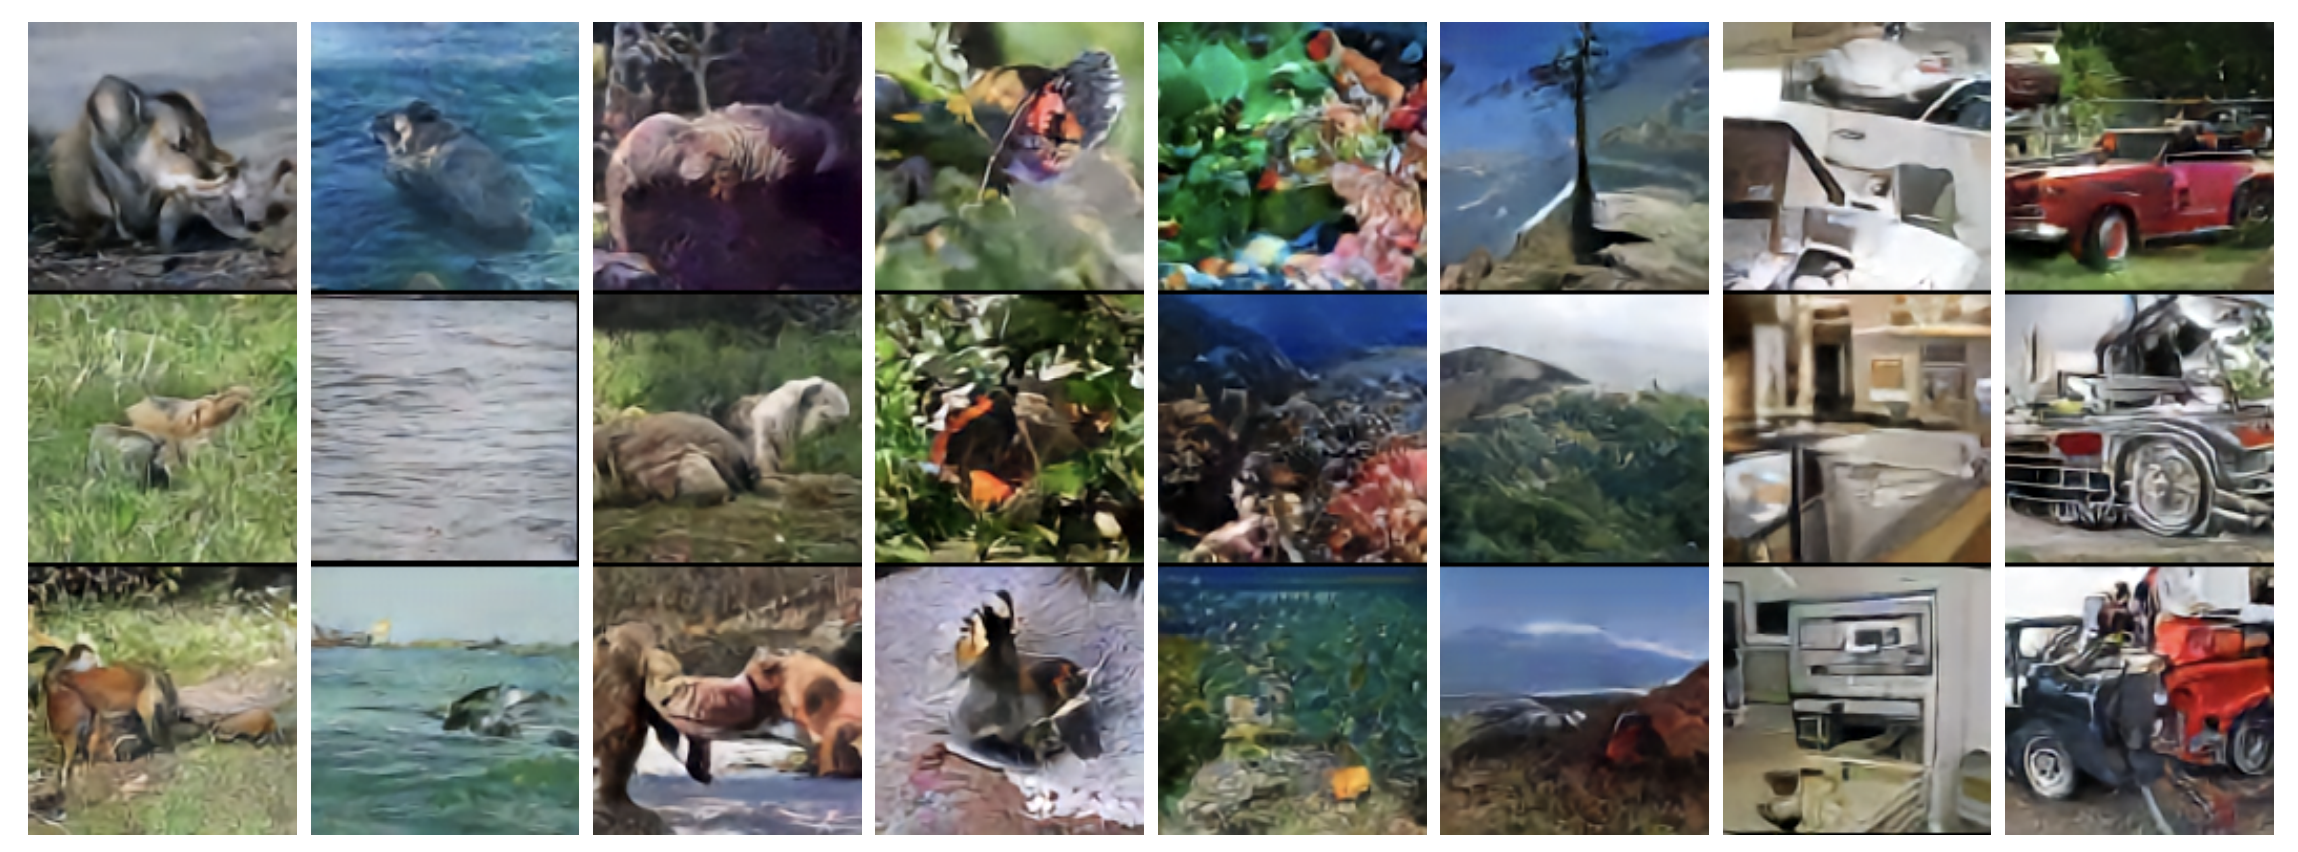
\includegraphics[width=\textwidth]{images/vqvae_samples.png}
    \caption{Samples generated by a VQ-VAE model \cite{vqvae}, trained on ImageNet dataset \cite{vqvae}.}
    \label{fig:vqvae_samples}
\end{figure}

We can see some generated samples created with VQ-VAE in figure \ref{fig:vqvae_samples}.








\subsection{Vector Quantization}
\label{vq}

Vector quantization (VQ) is a technique used to discretize continuous data. It allows the representation of a set of vectors using smaller set of representative vectors called \textbf{a codebook}. In a continuous latent space, the amount of possibilities for a value in the hidden space is infinite, which makes it \textbf{difficult for the model to learn the hidden space} efficiently.

We can see in figure \ref{fig:vqvae_cluster_visualization} an example of vector quantization in a 2D latent space. The red dots represent the codebook vectors, and the grey dots represent the embeddings of the continuous latent space. We cluster all the embeddings into the closest codebook vector, and the codebook vectors are the centroids of the clusters.

In the context of VQ-VAE, the continuous latent space $z$ is mapped into discrete codes vectors, and learning becomes more efficient because there is a fixed and smaller number of possible values in the latent space.

\begin{figure}[h]
    \centering
    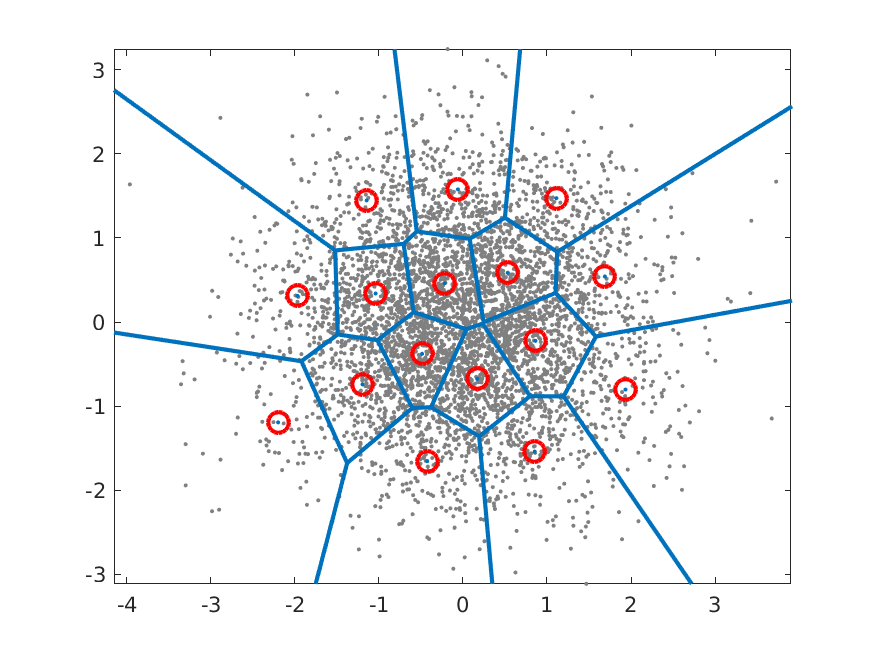
\includegraphics[scale=0.5]{images/vq_visualization.png}
    \caption{Vector quantization: discrete clustering of the 2D latent space. \textit{Grey dots}: embeddings of the continuous latent space. \textit{Red dots}: the codebook vectors. In this case, the codebook size is 16 (16 clusters) \cite{vq_visualization_website}.}
    \label{fig:vqvae_cluster_visualization}
\end{figure}

After the input passes through the encoder, the embeddings are replaced by the \textbf{closest vector from the codebook} (by minimizing distance between vectors, usually Euclidean distance). 

The input vectors are partitioned into clusters and each cluster is represented by a single codebook vector (see eq. \ref{eq:vq_onehot}):

\begin{equation}
    \label{eq:vq_onehot}
    q(z=k|x) = \begin{cases}
        1 & \text{if } \text{for } k=\text{argmin}_j \Vert z_e(x) - e_j \Vert_2 \\
        0 & \text{otherwise}
    \end{cases}
\end{equation}

Let $K$ be the size of the discrete latent space and $D$ the dimensionality of each latent embedding vector $e_i$. There are $K$ embedding vectors: $e_i \in \mathbb{R}^D, i \in 1, 2, ..., K$. The model takes an input $x$ (in the VQ-VAE paper \ref{vqvae} it was images) and is passed through an encoder, producing $z_e(x)$. The discrete latent variables $z$ are then calculated by a nearest neighbor look-up: $\text{argmin}_j \Vert z_e(x) - e_j \Vert_2$ which finds the index $k$ of the embedding vector $e_j$ closest to $z_e(x)$. 

% The input to the decoder is the vector $e_k$ in the following equation:

% \begin{equation}
%     z_q(x) = e_k,\ \text{where}\ k = \text{argmin}_j \Vert z_e(x) - e_j \Vert_2
% \end{equation}






\subsection{Architecture}

\begin{figure}[h]
    \centering
    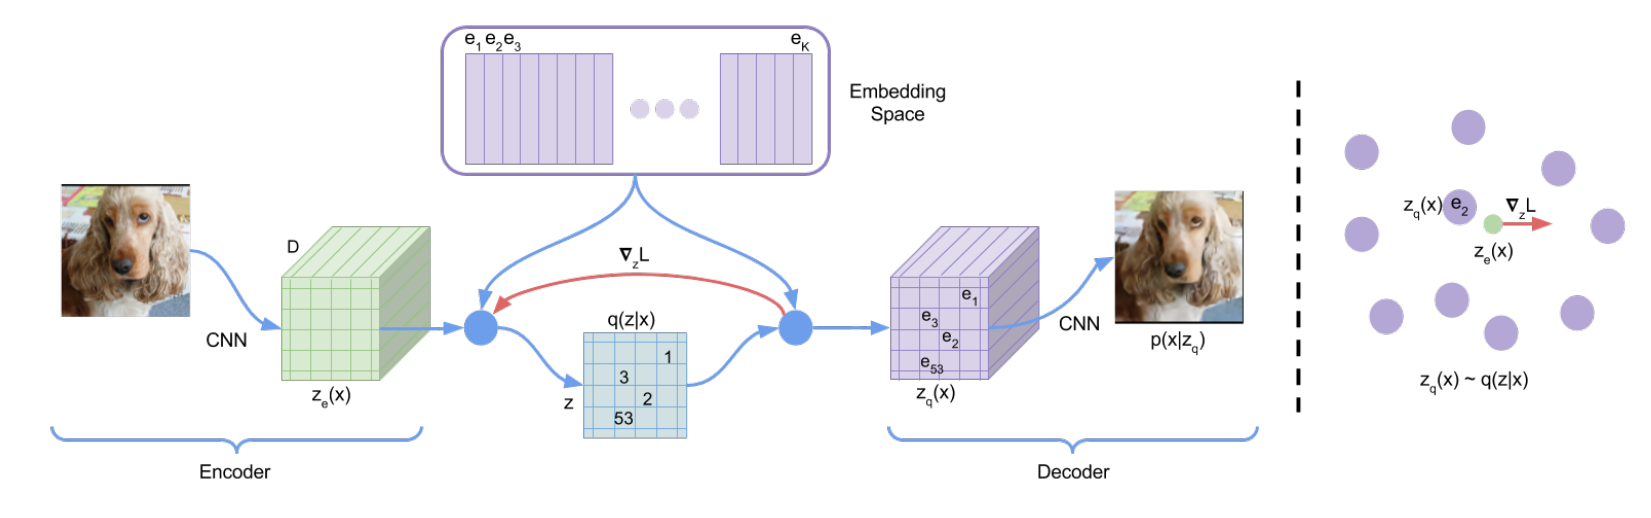
\includegraphics[width=\textwidth]{images/vqvae_architecture.png}
    \caption{VQ-VAE architecture \cite{vqvae}. \textit{Purple}: the code vectors. \textit{Green}: the embeddings before quantization. \textit{Blue}: the codebook indices (one-hot vectors). \textit{Right}: the 'snapping' operation which replaces the embeddings with the closest codebook vector \cite{vqvae}.}
    \label{fig:vqvae_architecture}
\end{figure}

The architecture of VQ-VAE is shown in figure \ref{fig:vqvae_architecture}. The model is similar in structure to VAE but with the addition of vector quantization component and the codebook embeddings.

The encoder first maps the input $x$ to a continuous latent space $z_e$ using CNN layers. The embeddings $z_e$ are then quantized to the nearest code vector in the codebook, resulting in the quantized embeddings $z_q$. These embeddings are passed to the decoder to reconstruct the image.

The quantization operation is not differentiable, that is why a straight-through estimator (STE) is used (see STE \ref{ste}) to allow backpropagation.







\subsection{Training}

The \textbf{codebook is learned} by minimizing the loss function:

\begin{equation}
    \mathcal{L}_{\text{VQ}} = || \text{sg}[z_e] - z_q ||_2^2 + \beta || \text{sg}[z_q] - z_e ||_2^2
\label{eq:vq_loss}
\end{equation}

where $z_e$ is the encoder output, $z_q$ is the quantized output, $\text{sg}[\cdot]$ is the \textbf{stop gradient operation} (which prevents gradients from flowing through the quantization operation), and $\beta$ is a hyperparameter that controls the weighting of the two terms in the loss function. 

The first term in the loss function is the \textbf{quantization loss}, which measures the distance between the encoder output and the quantized output. 

The second term is the \textbf{commitment loss}, which measures the distance between the quantized output and the encoder output. The commitment loss encourages the model to use the codebook, and prevents the model from ignoring the quantization operation.

\begin{equation}
    \label{eq:quantization}
    z_q(x)=e_k, \text{  where } k = \text{argmin}_j || z_e(x) - e_j ||_2
\end{equation}

Finding the nearest code vector in the codebook is given by equation \ref{eq:quantization}.

The \textbf{loss function of the VQ-VAE} is given by:

\begin{equation}
    \mathcal{L}_\text{VQ-VAE} = 
    \underbrace{\text{log } p(x|z_q(x))}_{\text{recon loss}} + 
    \underbrace{\Vert \text{sg}[z_e(x)] - e \Vert_2^2}_{\text{quant loss}} +
    \underbrace{\beta \Vert z_e(x) - \text{sg}[e] \Vert_2^2}_{\text{commit loss}}
    \label{eq:vqvae_loss}
\end{equation}
    
The decoder optimizes the first loss term only (reconstruction loss), the encoder optimizes the first and last loss (commitment loss) terms, and the embeddings are optimized in the middle term (quantization loss).






\subsection{Straight Through Estimator (STE)}
\label{ste}

Snapping embeddings to the nearest codebook vectors operation is not differentiable, which means the gradients will always be 0 at the backpropagation \cite{why_round_function_is_not_differentiable}.

The STE is a technique used to \textbf{approximate the gradients of a non-differentiable function} by passing the gradients of the function through the function itself (in other words, they skip the quantization operation in the backward pass):


% \begin{lstlisting}[language=Python, label=lst:vqvae_stop_gradients, caption=Allow gradients to flow through the snapping operation.]
%     # preserve gradients
%     z_q = z + (z_q - z).detach()
% \end{lstlisting}

In figure \ref{fig:vqvae_architecture} we can see the STE with the red arrow, which copy the gradients from the decoder to the encoder (and skips the quantization process, in the middle).






\subsection{Video Generation Experiment}

\begin{figure}[h]
    \centering
    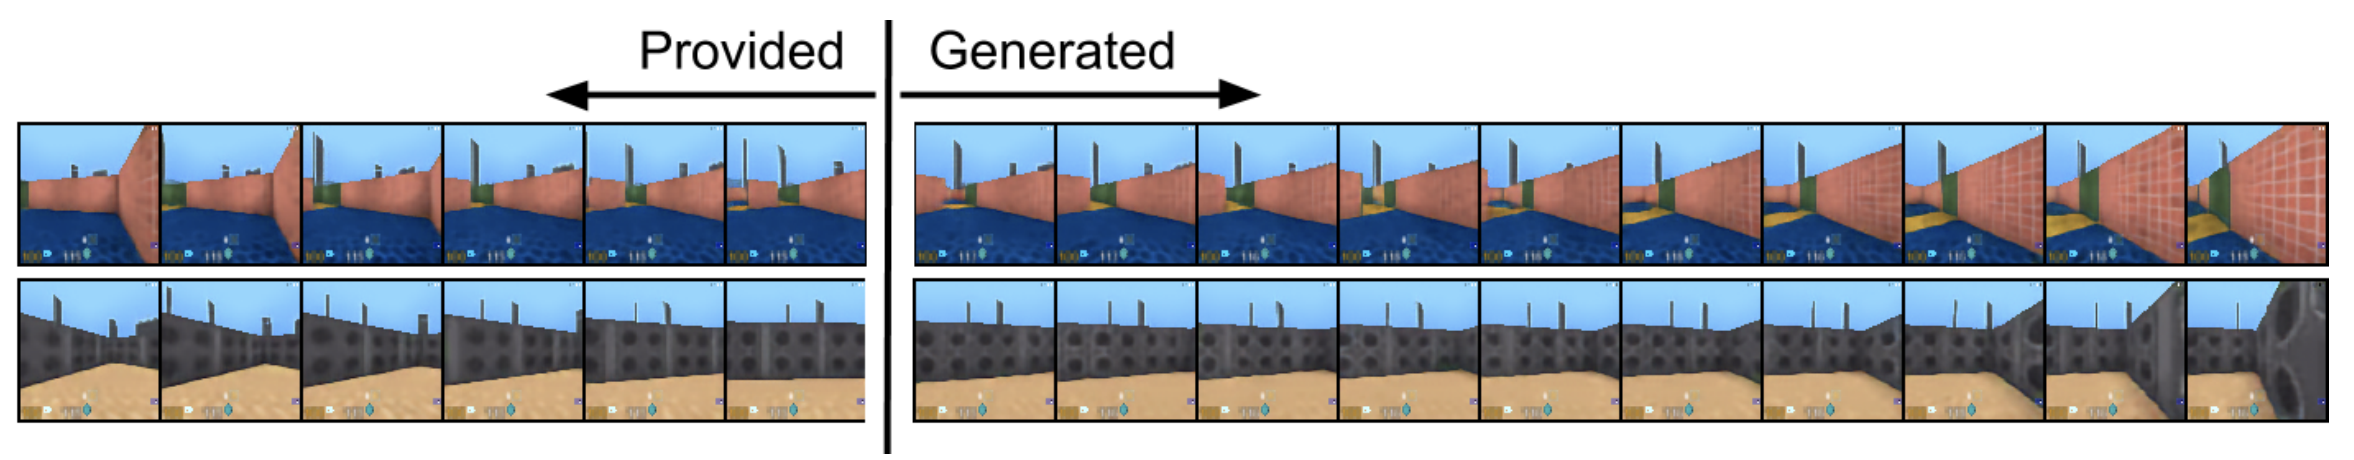
\includegraphics[width=\textwidth]{images/vqvae_video_generation.png}
    \caption{VQ-VAE video generation experiment \cite{vqvae}. \textit{Top}: the "move forward" action. \textit{Bottom}: the "move right" action \cite{vqvae}.}
    \label{fig:vqvae_video_generation}
\end{figure}

The researchers used the VQ-VAE model to generate videos conditioned on actions (video game controls). In figure \ref{fig:vqvae_video_generation} we can see the results of the video generation experiment. Given 6 frames as input, the model predicted the next 10 frames conditioned on the action. Each image is created by first generating latents and then ingress into the decoder.
